%Matteo Kumar - Leonhard Schatt
% Fortgeschrittenes Physikalisches Praktikum

% Teilauswertung Bleach

\section{Bestimmung der Förstereffizienz über Bleichung der Akzeptoren}

Ein alternativer Ansatz zur Bestimmung der Förstereffizienz $E$ ist, die Donorfluoreszenz vor und nach dem Bleichen der Akzeptoren zu betrachten. Denn wird ein 
Teil der Akzeptoren zerstört, so gibt es für einen Donor im angeregten Zustand nur noch einen möglichen Weg, diesen zu verlassen: Das angeregte Elektron relaxiert in den 
Grundzustand unter Aussendung eines Photons; es ist also eine Erhöhung der Donorfluoreszenz zu erwarten und zwar um den Betrag, um den die Sensitized Emission zurückgeht. \\
Um eine Zelle aus der Probe mit CFP und YFP wird eine ROI1 ausgewählt, die gebleicht werden soll. 
Zudem wird in dieser, wie auch in der Membranregion (ROI2) und in einer kleinen Region dieser (ROI3) die Intensität kurz vor bis kurz nach dem Bleichvorgang gemessen. 
In Abb. \ref{bild:bleachROI} ist so eine Zelle dargestellt. Dabei ist die ROI1 in Grün, ROI2 in Violett und ROI3 in Orange dargestellt. In Abb. \ref{bild:bleachPlotD} 
und Abb. \ref{bild:bleachPlotS} sind die Intensitätsverläufe dieser Zelle für den Donor- bzw. SE-Kanal in den selben Farben dargestellt. 
Dabei ist vor allem in den ROIs 2 ud 3, also in denjenigen, in denen die Dichte an Fluorophoren besonders groß ist, zu erkennen, dass zum 
Einen die Donorfluoreszenz nach dem Bleichen einen höheren Wert erreicht. Zum Anderen fällt dort die Intensität im SE-Kanal nach dem 
Bleichvorgang ab.


\begin{figure}[h]
    \centering
    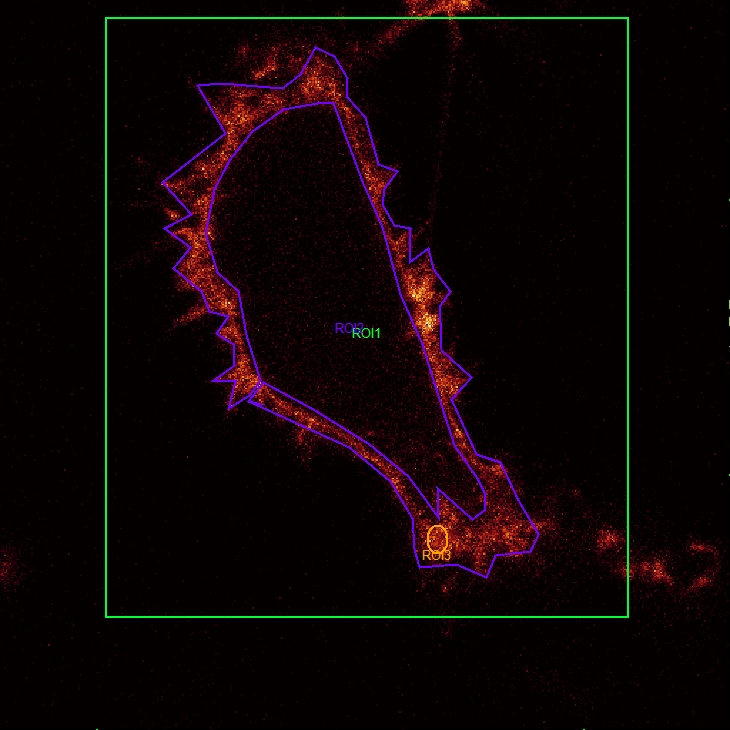
\includegraphics[scale = 0.55]{Bilder/bleachROI.jpg}
    \caption{Bild einer gebleichten Zelle mit CFP und YFP. Dabei sind die ROIs, in denen die Intensitäten gemessen wurden eingezeichnet.}
    \label{bild:bleachROI}
\end{figure}

\begin{figure}[h]
    \centering
    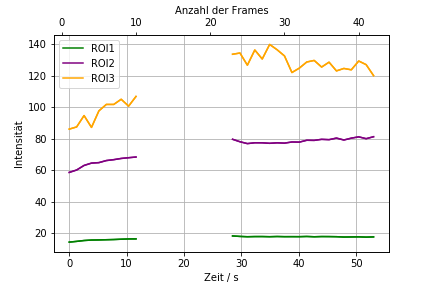
\includegraphics[scale = 0.65]{Bilder/bleachPlotD.png}
    \caption{Verlauf der Intensitäten einer Zelle mit CFP und YFP für verschiedenen ROIs im Donor-Kanal vor, während und nach dem Bleichen.}
    \label{bild:bleachPlotD}
\end{figure}

\begin{figure}[h]
    \centering
    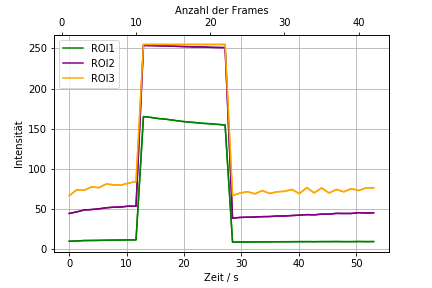
\includegraphics[scale = 0.65]{Bilder/bleachPlotS.png}
    \caption{Verlauf der Intensitäten einer Zelle mit CFP und YFP für verschiedenen ROIs im SE-Kanal vor, während und nach dem Bleichen.}
    \label{bild:bleachPlotS}
\end{figure}

Eine Abschätzung der Förstereffizienz $E$ ergibt sich laut S.9 des Praktikumskripts nach 
\begin{equation*}
    E = 1 - \frac{D_{CY,pre}}{D_{CY,post}},
\end{equation*}
wobei $D_{CY,pre}$ und $D_{CY,post}$ die Intensitäten im Donorkanal vor bzw. nach dem Bleichen sind. Für die Intensitäten werden die Mittelwerte 
für jede Zelle über die entsprechenden Messpunkte vor und nach dem Bleichen berechnet. Diese Werte und die daraus resultierenden Werte 
für $E$ finden sich in Tab. \ref{tab:bleach}.

\begin{center}
    \centering
    \begin{tabular}{lrrrrrrrrr}
        \toprule
        Nr &   $D_{pre,ROI1}$ &  $D_{post,ROI1}$ &   $D_{pre,ROI2}$ &  $D_{post,ROI2}$ &    $D_{pre,ROI3}$ &   $D_{post,ROI3}$ &     $E_{ROI1}$ &    $E_{ROI2}$ &    $E_{ROI3}$ \\
        \midrule
        1  & 16,235 & 15,317 & 33,497 & 34,979 &  77,237 &  90,776 & -0,060 & 0,042 & 0,149 \\
        2  & 13,066 & 14,249 & 63,486 & 78,032 &  76,281 & 161,321 &  0,083 & 0,186 & 0,527 \\
        3  & 10,776 & 11,753 & 37,788 & 56,380 &  28,369 &  95,764 &  0,083 & 0,330 & 0,704 \\
        4  & 16,744 & 19,713 & 49,572 & 60,298 &  93,544 & 128,803 &  0,151 & 0,178 & 0,274 \\
        5  & 24,869 & 27,825 & 78,394 & 99,958 &  89,080 & 163,331 &  0,106 & 0,216 & 0,455 \\
        6 & 14,541 & 16,041 & 44,807 & 51,012 &  76,670 & 101,924 &  0,093 & 0,122 & 0,248 \\
        7 & 20,765 & 23,984 & 71,346 & 86,995 & 102,374 & 133,280 &  0,134 & 0,180 & 0,232 \\
        8 & 19,589 & 22,940 & 49,402 & 60,320 &  53,432 &  99,013 &  0,146 & 0,181 & 0,460 \\
        9 & 24,573 & 31,952 & 60,412 & 87,938 &  74,175 & 109,517 &  0,231 & 0,313 & 0,323 \\
        10 & 15,758 & 17,943 & 54,063 & 63,678 & 139,174 & 173,205 &  0,122 & 0,151 & 0,196 \\
        11 & 15,759 & 17,894 & 64,824 & 78,855 &  96,956 & 128,896 &  0,119 & 0,178 & 0,248 \\
        \bottomrule
    \end{tabular}
    \captionof{table}{Werte für die mittleren Intensitäten des Donorkanals vor und nach dem Bleichprozess für die verschiedenen ROIs 
    und die daraus berechneten Förstereffizienzen für Zellen mit CFP und YFP}
    \label{tab:bleach}
\end{center}

Nachdem ROI1 nicht nur die Zellmembran enthält, sollten die Werte für $E$ dort nicht sehr genau sein. Für Zelle 1 ist sogar ein negativer Wert 
zu erkennen. Die Werte von ROI2 und ROI3 unterscheiden sich auch deutlich; letzterer ist in der Regel deutlich höher. Das liegt daran, 
dass die Dichte der Flourophore nicht gleichmäßig über die Membran verteilt ist. $E$ in ROI2, der kompletten Membranregion, stellt also 
gewissermaßen einen Mittelwert für die Membran da. Dagegen wurde für ROI3 ein besonders heller Fleck im Bild ausgesucht, das heißt ein 
Ort mit hoher Intensität, was einer höheren Förstereffizienz entspricht. Man könnte den Wert für $E$ in ROI3 also als eine Art 
maximale Förstereffizienz in dieser Zelle betrachten; vorausgesetzt es wurde tatsächlich eine der hellsten Gebiete ausgewählt. 
Betrachtet man die Werte für $E$ in ROI2 (die "Mittelwerte" über die Membran), so liegen dort Effizienzen von 4,2\% bis 33\% vor. Ersterer 
erscheint zwar etwas niedrig, alle anderen jedoch liegen in etwa dem Bereich, in dem auch die Werte liegen, die in Abschnitt \ref{sec:SE} 
über die Sensitized Emission bestimmt wurden.\\
Betrachten wir nun eine Probe nur mit CFP, erwarten wir, dass bei Bleichung im Wellenbereich des Akzeptors kaum eine Veränderung der 
Intensitäten zu beobachten ist. In Tab. \ref{tab:bleachCFPd} sind die zugehörigen Intensitätsmittelwerte 
vor und nach dem Bleichen dargestellt für den Donorkanal. An den dort gelisteten Werten und an der graphischen Auftragung 
dieser und denen für den SE-Kanal für eine bestimmte Zelle in Abb. \ref{bild:bleachCFPd} und \ref{bild:bleachCFPs} ist zwar ein leichter Anstieg der INtensitäten 
nach dem Bleichen zu erkennen; dieser fällt jedoch im Vergleich zu dem für die CFP/YFP-Probe wesentlich geringer aus.

\begin{center}
    \centering
    \begin{tabular}{lrrrrrr}
        \toprule
        Zelle &   $D_{pre,ROI1}$ &  $D_{post,ROI1}$ &   $D_{pre,ROI2}$ &  $D_{post,ROI2}$ &    $D_{pre,ROI3}$ &   $D_{post,ROI3}$ \\ 
        \midrule
        1 & 26,782 & 28,486 &  88,599 &  98,089 & 135,201 & 160,823 \\
        2 & 21,599 & 22,385 & 111,558 & 116,090 & 139,774 & 160,140 \\
        3 & 36,387 & 39,985 & 129,027 & 143,848 & 136,273 & 164,422 \\
        4 & 39,784 & 43,081 & 124,343 & 140,135 & 180,502 & 225,815 \\
        5 & 35,197 & 35,784 & 148,151 & 153,460 & 177,970 & 206,161 \\
        \bottomrule
    \end{tabular}
    \captionof{table}{Mittelwerte der Intensitäten einer Zelle mit ausschließlich CFP vor und nach dem Bleichen in verschiedenen ROIs}
    \label{tab:bleachCFPd}
\end{center}

\begin{figure}[h]
    \centering
    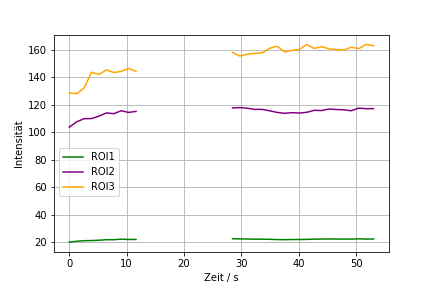
\includegraphics[scale = 0.65]{Bilder/bleachPlotCFPd.png}
    \caption{Verlauf der Intensitäten einer Zelle mit ausschließlich CFP für verschiedenen ROIs im Donorkanal vor, während und nach dem Bleichen.}
    \label{bild:bleachCFPd}
\end{figure}

\begin{figure}[h]
    \centering
    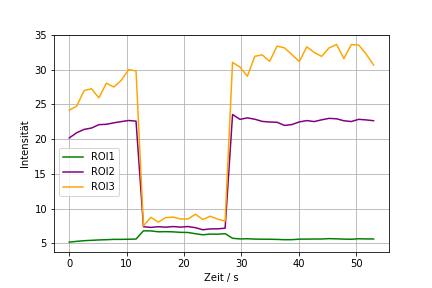
\includegraphics[scale = 0.65]{Bilder/bleachPlotCFPs.png}
    \caption{Verlauf der Intensitäten einer Zelle mit ausschließlich CFP für verschiedenen ROIs im SE-Kanal vor, während und nach dem Bleichen.}
    \label{bild:bleachCFPs}
\end{figure}

Betrachtet man nun eine reine YFP-Probe, deren Intensitäten vor und nach dem Bleichen in Tab. \ref{tab:bleachYFP} zu finden sind, so 
ist hier eine deutliche Abnahme der Intensität zu beobachten, welche auch gut in der graphischen Auftragung für eine Zelle in Abb. 
\ref{bild:blachYFP} zu erkennen ist. Dies ist auch zu erwarten, da durch das Bleichen etliche der YFP zerstört werden, da die Wellenlänge 
des Lasers zu dem Anregungsspektrum des YFP passt.

\begin{center}
    \centering
    \begin{tabular}{lrrrrrr}
        \toprule
        Zelle &   $A_{pre,ROI1}$ &  $A_{post,ROI1}$ &   $A_{pre,ROI2}$ &  $A_{post,ROI2}$ &    $A_{pre,ROI3}$ &   $A_{post,ROI3}$ \\
        \midrule
        1 & 11,416 &  9,638 &  60,466 & 50,968 & 141,574 & 119,333 \\
        2 & 14,750 & 10,965 &  67,742 & 48,875 & 124,682 &  96,868 \\
        3 & 22,750 & 10,951 & 116,744 & 48,890 & 154,576 &  62,938 \\
        4 & 22,859 & 10,623 &  92,145 & 47,088 & 128,689 &  90,851 \\
        5 & 16,507 &  8,019 &  75,914 & 34,303 & 162,438 &  64,721 \\
        \bottomrule
    \end{tabular}
    \captionof{table}{Werte für die Intensitäten im Akzeptorkanal vor und nach dem Bleichen einer Probe mit reinem YFP 
    in verschiedenen ROIs. Dabei ist eine deutliche Abnahme über den Bleichprozess hinweg zu beobachten.}
    \label{tab:bleachYFP}
\end{center}

\begin{figure}[h]
    \centering
    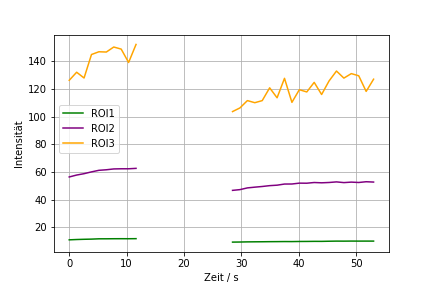
\includegraphics[scale = 0.65]{Bilder/bleachPlotYFP.png}
    \caption{Verlauf der Intensitäten einer Zelle mit ausschließlich YFP für verschiedenen ROIs im Akzeptorkanal vor, während und 
    nach dem Bleichen. Auch hier ist die Abnahme über den Bleichprozess deutlich zu sehen.}
    \label{bild:bleachCFPs}
\end{figure}

\clearpage